\documentclass[12pt]{article}
\usepackage{fullpage,enumitem,amsmath,amssymb,graphicx}
\usepackage{graphicx} % This is a package for including graphics in your solution.
\usepackage{listings}
\usepackage[final]{pdfpages}

\begin{document}

\begin{center}
{\Large CS168 Spring Assignment 2}

\begin{tabular}{rl}
SUNet ID(s): 05794739 & \\
Name(s): & Luis A. Perez \\
Collaborators: &
\end{tabular}
\end{center}

By turning in this assignment, I agree by the Stanford honor code and declare
that all of this is my own work.

\section*{Part 1}

\begin{enumerate}[label=(\alph*)]
  \item
    \begin{verbatim}
import collections
import matplotlib.pyplot as plt

import numpy as np
import pandas as pd
import seaborn as sns
import os
import warnings

from typing import Dict, List, Text, Tuple

# Make figure larger
plt.rcParams['figure.figsize'] = [10, 5]

class Globals:
    """Class holding globals to avoid polluting workspace."""
    DATA_DIR: Text = 'p2_data'
    LABEL: Text = 'label.csv'
    GROUPS: Text = 'groups.csv'
    DATA: Text = 'data50.csv'

def makeHeatMap(data, names, color, outputFileName):
    """Makes a 20x20 heatmap from the given 20x20 data matrix."""
    # to catch "falling back to Agg" warning
    with warnings.catch_warnings():
        warnings.simplefilter("ignore")
        # code source: http://stackoverflow.com/questions/14391959/heatmap-in-matplotlib-with-pcolor
        fig, ax = plt.subplots()
        # create the map w/ color bar legend
        heatmap = ax.pcolor(data, cmap=color)
        cbar = plt.colorbar(heatmap)

        # put the major ticks at the middle of each cell
        ax.set_xticks(np.arange(data.shape[0]) + 0.5, minor=False)
        ax.set_yticks(np.arange(data.shape[1]) + 0.5, minor=False)

        # want a more natural, table-like display
        ax.invert_yaxis()
        ax.xaxis.tick_top()

        ax.set_xticklabels(range(1, 21))
        ax.set_yticklabels(names)

        plt.tight_layout()

        plt.savefig(outputFileName, format='png')
        plt.close()

def get_bag_of_words(data: pd.DataFrame) -> collections.Counter:
    """Transforms a pandas dataframe into a bag of words counter.
    
    Args:
        data, with columns 'wordId' and 'count'
        
    Returns:
        The bag of words (mapping from wordId to count).
    """
    return collections.Counter({
        wordId: count for wordId, count in zip(data.wordId, data['count'])})
        
def read_data() -> Tuple[Dict[int, int], Dict[int, List[int]], pd.DataFrame]:
    """Reads the relevant data files.
    
    Returns:
        A tuple of items. The bag of words object and for each 
        article (keyed by articleId) and a mapping from
        groupId to a list of corresponding articleIds in that group.
        Also the entire dataset as a pd.DataFrame.
    """
    # Maps to groupId.
    labels = pd.read_csv(
        os.path.join(Globals.DATA_DIR, Globals.LABEL), header=None,
        names=['groupId'])
    labels['articleId'] = range(1, len(labels) + 1)
    # Maps to groupName.
    groups = pd.read_csv(
        os.path.join(Globals.DATA_DIR,
                     Globals.GROUPS), header=None,
        names=['name'])
    groups['groupId'] = range(1, len(groups) + 1)
    data = pd.read_csv(
        os.path.join(Globals.DATA_DIR, Globals.DATA), header=None,
        names=['articleId', 'wordId', 'count'])
    data = data.merge(labels, on='articleId').merge(groups, on='groupId')
    # Transform into a dictionary mapping articleId to a collections.Counter
    # object counting each word (based on wordId).
    group_to_name = {groupId : data[data.groupId == groupId].name.iloc[0]
                    for groupId in data.groupId.unique()}
    article_to_bow = {articleId : get_bag_of_words(data[data.articleId == articleId])
            for articleId in data.articleId.unique()}
    group_to_article = { groupId : data[data.groupId == groupId].articleId.unique()
                       for groupId in data.groupId.unique()}
    return article_to_bow, group_to_article, group_to_name   

def jaccard_sim(x: Dict[int, int], y: Dict[int, int]) -> float:
    """Given two bag-of-word representations, calculate their Jaccard Similarity."""
    num = 0
    den = 0
    for wordId in (set(x.keys()) | set(y.keys())):
        num += min(x[wordId], y[wordId])
        den += max(x[wordId], y[wordId])
    return num / den

def lp_sim(x: Dict[int, int], y: Dict[int, int], p: int = 2) -> float:
    """Given two bag-of-word representations, calculate their l_p norm similarity."""
    squaredSum = 0
    for wordId in (set(x.keys()) | set(y.keys())):
        squaredSum += (x[wordId] - y[wordId])**p
    return -np.sqrt(squaredSum)

def cosine_sim(x: Dict[int, int], y: Dict[int, int]) -> float:
    """Given two bag-of-word representations, calculate their cosine similarity."""
    xNorm = np.linalg.norm(list(x.values()))
    yNorm = np.linalg.norm(list(y.values()))
    dotProduct = 0
    for wordId in (set(x.keys()) | set(y.keys())):
        dotProduct += (x[wordId] * y[wordId])
    return dotProduct / (xNorm * yNorm)

def average_similarity(articles, groups_to_articles, sim_fn, groupA: int, groupB: int) -> float:
    """Computes the average similarity between the two specified groups."""
    articlesA = groups_to_articles[groupA]
    articlesB = groups_to_articles[groupB]
    # Even though all of our existing sim_fn are symmetric, do
    # all pairs in-case this doesn't hold true in general.
    scores = [sim_fn(articles[Aidx], articles[Bidx])
              for Aidx in articlesA for Bidx in articlesB]
    return np.mean(scores)

def get_similarity_matrix(articles, groups_to_articles, sim_fn, max_groups=None):
    """Computes the similarity matrix using the given sim_fn for all groups."""
    groups = sorted(groups_to_articles.keys())
    if not max_groups: max_groups = len(groups)
    data = np.zeros((20,20))
    for i, groupA in enumerate(groups[:max_groups]):
        for j, groupB in enumerate(groups[:max_groups]):
            data[i][j] = average_similarity(
                articles, groups_to_articles, sim_fn, groupA, groupB)
    return data

def get_all_sim_matrices(articles, groups_to_articles, sim_fns):
    """Computes all similarity matrices for all given sim_fns."""
    data = {}
    for name, sim_fn in sim_fns.items():
        data[name] = get_similarity_matrix(articles, groups_to_articles, sim_fn)
    return data

def plot_heatmaps(input_data, sim_fns):
    """Plots and saves heatmaps for different similarity functions."""
    articles, groups_to_articles, group_names = input_data
    names = [group_names[i] for i in sorted(group_names.keys())]
    all_data = get_all_sim_matrices(articles, groups_to_articles, sim_fns)
    for name, data in all_data.items():
        makeHeatMap(data, names, color='Blues',
                    outputFileName="figures/{name}.png".format(name=name))

def problem_2b():
    """Solves problem 2b from Mini-Project 2"""
    input_data = read_data()
    plot_heatmaps(input_data, {
        'Cosine' : cosine_sim,
        'Jaccard': jaccard_sim,
        'L2' : lp_sim })

problem_2b()
    \end{verbatim}
  \item
    We now show the heat maps for each of the above strategies.

    \begin{figure}[!ht]
      \centering
      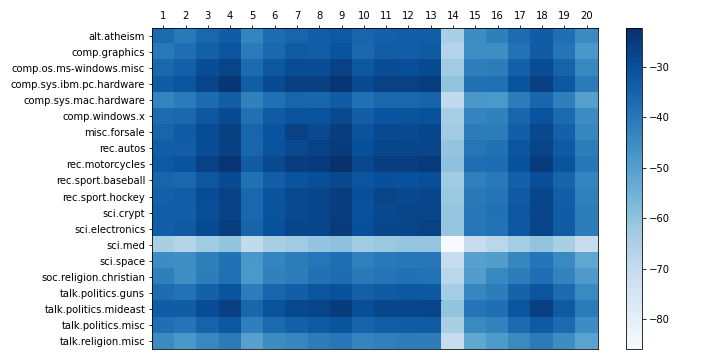
\includegraphics[scale=0.6]{figures/L2.png}
      \begin{caption}
        L2 Similarity Metric Heat Map.
      \end{caption}
    \end{figure}
    \begin{figure}[!ht]
      \centering
      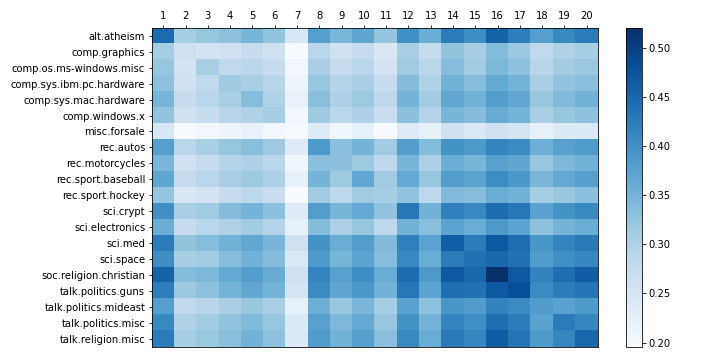
\includegraphics[scale=0.6]{figures/Cosine.png}
      \begin{caption}
        Cosine Similarity Metric Heat Map.
      \end{caption}
    \end{figure}
    \begin{figure}[!ht]
      \centering
      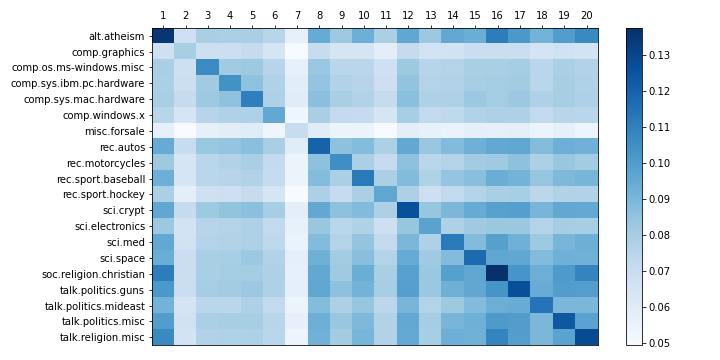
\includegraphics[scale=0.6]{figures/Jaccard.png}
      \begin{caption}
        Jaccard Similarity Metric Heat Map.
      \end{caption}
    \end{figure}
\end{enumerate}

\section*{Part 2}

\begin{enumerate}[label=(\alph*)]
  \item (your solution, with code)
\begin{verbatim}
def cow():
    print ``Moo''
\end{verbatim}

  \item (your solution)
\end{enumerate}

\end{document}
